\documentclass[a4paper, 12pt]{article}
\usepackage[left=2cm,right=2cm, top=2cm,bottom=2cm,bindingoffset=0cm]{geometry}
\usepackage{cmap, amssymb, amsmath, amsthm, mathtools}
\usepackage{upgreek}
\usepackage{setspace}

    \usepackage[breakable]{tcolorbox}
    \usepackage{parskip} % Stop auto-indenting (to mimic markdown behaviour)
    

    % Basic figure setup, for now with no caption control since it's done
    % automatically by Pandoc (which extracts ![](path) syntax from Markdown).
    \usepackage{graphicx}
    % Keep aspect ratio if custom image width or height is specified
    \setkeys{Gin}{keepaspectratio}
    % Maintain compatibility with old templates. Remove in nbconvert 6.0
    \let\Oldincludegraphics\includegraphics
    % Ensure that by default, figures have no caption (until we provide a
    % proper Figure object with a Caption API and a way to capture that
    % in the conversion process - todo).
    \usepackage{caption}
    \DeclareCaptionFormat{nocaption}{}
    \captionsetup{format=nocaption,aboveskip=0pt,belowskip=0pt}

    \usepackage{float}
    \floatplacement{figure}{H} % forces figures to be placed at the correct location
    \usepackage{xcolor} % Allow colors to be defined
    \usepackage{enumerate} % Needed for markdown enumerations to work
    \usepackage{geometry} % Used to adjust the document margins
    \usepackage{amsmath} % Equations
    \usepackage{amssymb} % Equations
    \usepackage{textcomp} % defines textquotesingle
    % Hack from http://tex.stackexchange.com/a/47451/13684:
    \AtBeginDocument{%
        \def\PYZsq{\textquotesingle}% Upright quotes in Pygmentized code
    }
    \usepackage{upquote} % Upright quotes for verbatim code
    \usepackage{eurosym} % defines \euro

    \usepackage{iftex}
    \ifPDFTeX
        \usepackage[T2A]{fontenc}
        \IfFileExists{alphabeta.sty}{
              \usepackage{alphabeta}
          }{
              \usepackage[mathletters]{ucs}
              \usepackage[utf8]{inputenc}
          }
    \else
        \usepackage{fontspec}
        \usepackage{unicode-math}
    \fi

    \usepackage{fancyvrb} % verbatim replacement that allows latex
    \usepackage{grffile} % extends the file name processing of package graphics
                         % to support a larger range
    \makeatletter % fix for old versions of grffile with XeLaTeX
    \@ifpackagelater{grffile}{2019/11/01}
    {
      % Do nothing on new versions
    }
    {
      \def\Gread@@xetex#1{%
        \IfFileExists{"\Gin@base".bb}%
        {\Gread@eps{\Gin@base.bb}}%
        {\Gread@@xetex@aux#1}%
      }
    }
    \makeatother
    \usepackage[Export]{adjustbox} % Used to constrain images to a maximum size
    \adjustboxset{max size={0.9\linewidth}{0.9\paperheight}}

    % The hyperref package gives us a pdf with properly built
    % internal navigation ('pdf bookmarks' for the table of contents,
    % internal cross-reference links, web links for URLs, etc.)
    \usepackage{hyperref}
    % The default LaTeX title has an obnoxious amount of whitespace. By default,
    % titling removes some of it. It also provides customization options.
    \usepackage{titling}
    \usepackage{longtable} % longtable support required by pandoc >1.10
    \usepackage{booktabs}  % table support for pandoc > 1.12.2
    \usepackage{array}     % table support for pandoc >= 2.11.3
    \usepackage{calc}      % table minipage width calculation for pandoc >= 2.11.1
    \usepackage[inline]{enumitem} % IRkernel/repr support (it uses the enumerate* environment)
    \usepackage[normalem]{ulem} % ulem is needed to support strikethroughs (\sout)
                                % normalem makes italics be italics, not underlines
    \usepackage{soul}      % strikethrough (\st) support for pandoc >= 3.0.0
    \usepackage{mathrsfs}
    

    
    % Colors for the hyperref package
    \definecolor{urlcolor}{rgb}{0,.145,.698}
    \definecolor{linkcolor}{rgb}{.71,0.21,0.01}
    \definecolor{citecolor}{rgb}{.12,.54,.11}

    % ANSI colors
    \definecolor{ansi-black}{HTML}{3E424D}
    \definecolor{ansi-black-intense}{HTML}{282C36}
    \definecolor{ansi-red}{HTML}{E75C58}
    \definecolor{ansi-red-intense}{HTML}{B22B31}
    \definecolor{ansi-green}{HTML}{00A250}
    \definecolor{ansi-green-intense}{HTML}{007427}
    \definecolor{ansi-yellow}{HTML}{DDB62B}
    \definecolor{ansi-yellow-intense}{HTML}{B27D12}
    \definecolor{ansi-blue}{HTML}{208FFB}
    \definecolor{ansi-blue-intense}{HTML}{0065CA}
    \definecolor{ansi-magenta}{HTML}{D160C4}
    \definecolor{ansi-magenta-intense}{HTML}{A03196}
    \definecolor{ansi-cyan}{HTML}{60C6C8}
    \definecolor{ansi-cyan-intense}{HTML}{258F8F}
    \definecolor{ansi-white}{HTML}{C5C1B4}
    \definecolor{ansi-white-intense}{HTML}{A1A6B2}
    \definecolor{ansi-default-inverse-fg}{HTML}{FFFFFF}
    \definecolor{ansi-default-inverse-bg}{HTML}{000000}

    % common color for the border for error outputs.
    \definecolor{outerrorbackground}{HTML}{FFDFDF}

    % commands and environments needed by pandoc snippets
    % extracted from the output of `pandoc -s`
    \providecommand{\tightlist}{%
      \setlength{\itemsep}{0pt}\setlength{\parskip}{0pt}}
    \DefineVerbatimEnvironment{Highlighting}{Verbatim}{commandchars=\\\{\}}
    % Add ',fontsize=\small' for more characters per line
    \newenvironment{Shaded}{}{}
    \newcommand{\KeywordTok}[1]{\textcolor[rgb]{0.00,0.44,0.13}{\textbf{{#1}}}}
    \newcommand{\DataTypeTok}[1]{\textcolor[rgb]{0.56,0.13,0.00}{{#1}}}
    \newcommand{\DecValTok}[1]{\textcolor[rgb]{0.25,0.63,0.44}{{#1}}}
    \newcommand{\BaseNTok}[1]{\textcolor[rgb]{0.25,0.63,0.44}{{#1}}}
    \newcommand{\FloatTok}[1]{\textcolor[rgb]{0.25,0.63,0.44}{{#1}}}
    \newcommand{\CharTok}[1]{\textcolor[rgb]{0.25,0.44,0.63}{{#1}}}
    \newcommand{\StringTok}[1]{\textcolor[rgb]{0.25,0.44,0.63}{{#1}}}
    \newcommand{\CommentTok}[1]{\textcolor[rgb]{0.38,0.63,0.69}{\textit{{#1}}}}
    \newcommand{\OtherTok}[1]{\textcolor[rgb]{0.00,0.44,0.13}{{#1}}}
    \newcommand{\AlertTok}[1]{\textcolor[rgb]{1.00,0.00,0.00}{\textbf{{#1}}}}
    \newcommand{\FunctionTok}[1]{\textcolor[rgb]{0.02,0.16,0.49}{{#1}}}
    \newcommand{\RegionMarkerTok}[1]{{#1}}
    \newcommand{\ErrorTok}[1]{\textcolor[rgb]{1.00,0.00,0.00}{\textbf{{#1}}}}
    \newcommand{\NormalTok}[1]{{#1}}

    % Additional commands for more recent versions of Pandoc
    \newcommand{\ConstantTok}[1]{\textcolor[rgb]{0.53,0.00,0.00}{{#1}}}
    \newcommand{\SpecialCharTok}[1]{\textcolor[rgb]{0.25,0.44,0.63}{{#1}}}
    \newcommand{\VerbatimStringTok}[1]{\textcolor[rgb]{0.25,0.44,0.63}{{#1}}}
    \newcommand{\SpecialStringTok}[1]{\textcolor[rgb]{0.73,0.40,0.53}{{#1}}}
    \newcommand{\ImportTok}[1]{{#1}}
    \newcommand{\DocumentationTok}[1]{\textcolor[rgb]{0.73,0.13,0.13}{\textit{{#1}}}}
    \newcommand{\AnnotationTok}[1]{\textcolor[rgb]{0.38,0.63,0.69}{\textbf{\textit{{#1}}}}}
    \newcommand{\CommentVarTok}[1]{\textcolor[rgb]{0.38,0.63,0.69}{\textbf{\textit{{#1}}}}}
    \newcommand{\VariableTok}[1]{\textcolor[rgb]{0.10,0.09,0.49}{{#1}}}
    \newcommand{\ControlFlowTok}[1]{\textcolor[rgb]{0.00,0.44,0.13}{\textbf{{#1}}}}
    \newcommand{\OperatorTok}[1]{\textcolor[rgb]{0.40,0.40,0.40}{{#1}}}
    \newcommand{\BuiltInTok}[1]{{#1}}
    \newcommand{\ExtensionTok}[1]{{#1}}
    \newcommand{\PreprocessorTok}[1]{\textcolor[rgb]{0.74,0.48,0.00}{{#1}}}
    \newcommand{\AttributeTok}[1]{\textcolor[rgb]{0.49,0.56,0.16}{{#1}}}
    \newcommand{\InformationTok}[1]{\textcolor[rgb]{0.38,0.63,0.69}{\textbf{\textit{{#1}}}}}
    \newcommand{\WarningTok}[1]{\textcolor[rgb]{0.38,0.63,0.69}{\textbf{\textit{{#1}}}}}


    % Define a nice break command that doesn't care if a line doesn't already
    % exist.
    \def\br{\hspace*{\fill} \\* }
    % Math Jax compatibility definitions
    \def\gt{>}
    \def\lt{<}
    \let\Oldtex\TeX
    \let\Oldlatex\LaTeX
    \renewcommand{\TeX}{\textrm{\Oldtex}}
    \renewcommand{\LaTeX}{\textrm{\Oldlatex}}
    % Document parameters
    % Document title
    \title{notebook}
    
    
    
    
    
    
    
% Pygments definitions
\makeatletter
\def\PY@reset{\let\PY@it=\relax \let\PY@bf=\relax%
    \let\PY@ul=\relax \let\PY@tc=\relax%
    \let\PY@bc=\relax \let\PY@ff=\relax}
\def\PY@tok#1{\csname PY@tok@#1\endcsname}
\def\PY@toks#1+{\ifx\relax#1\empty\else%
    \PY@tok{#1}\expandafter\PY@toks\fi}
\def\PY@do#1{\PY@bc{\PY@tc{\PY@ul{%
    \PY@it{\PY@bf{\PY@ff{#1}}}}}}}
\def\PY#1#2{\PY@reset\PY@toks#1+\relax+\PY@do{#2}}

\@namedef{PY@tok@w}{\def\PY@tc##1{\textcolor[rgb]{0.73,0.73,0.73}{##1}}}
\@namedef{PY@tok@c}{\let\PY@it=\textit\def\PY@tc##1{\textcolor[rgb]{0.24,0.48,0.48}{##1}}}
\@namedef{PY@tok@cp}{\def\PY@tc##1{\textcolor[rgb]{0.61,0.40,0.00}{##1}}}
\@namedef{PY@tok@k}{\let\PY@bf=\textbf\def\PY@tc##1{\textcolor[rgb]{0.00,0.50,0.00}{##1}}}
\@namedef{PY@tok@kp}{\def\PY@tc##1{\textcolor[rgb]{0.00,0.50,0.00}{##1}}}
\@namedef{PY@tok@kt}{\def\PY@tc##1{\textcolor[rgb]{0.69,0.00,0.25}{##1}}}
\@namedef{PY@tok@o}{\def\PY@tc##1{\textcolor[rgb]{0.40,0.40,0.40}{##1}}}
\@namedef{PY@tok@ow}{\let\PY@bf=\textbf\def\PY@tc##1{\textcolor[rgb]{0.67,0.13,1.00}{##1}}}
\@namedef{PY@tok@nb}{\def\PY@tc##1{\textcolor[rgb]{0.00,0.50,0.00}{##1}}}
\@namedef{PY@tok@nf}{\def\PY@tc##1{\textcolor[rgb]{0.00,0.00,1.00}{##1}}}
\@namedef{PY@tok@nc}{\let\PY@bf=\textbf\def\PY@tc##1{\textcolor[rgb]{0.00,0.00,1.00}{##1}}}
\@namedef{PY@tok@nn}{\let\PY@bf=\textbf\def\PY@tc##1{\textcolor[rgb]{0.00,0.00,1.00}{##1}}}
\@namedef{PY@tok@ne}{\let\PY@bf=\textbf\def\PY@tc##1{\textcolor[rgb]{0.80,0.25,0.22}{##1}}}
\@namedef{PY@tok@nv}{\def\PY@tc##1{\textcolor[rgb]{0.10,0.09,0.49}{##1}}}
\@namedef{PY@tok@no}{\def\PY@tc##1{\textcolor[rgb]{0.53,0.00,0.00}{##1}}}
\@namedef{PY@tok@nl}{\def\PY@tc##1{\textcolor[rgb]{0.46,0.46,0.00}{##1}}}
\@namedef{PY@tok@ni}{\let\PY@bf=\textbf\def\PY@tc##1{\textcolor[rgb]{0.44,0.44,0.44}{##1}}}
\@namedef{PY@tok@na}{\def\PY@tc##1{\textcolor[rgb]{0.41,0.47,0.13}{##1}}}
\@namedef{PY@tok@nt}{\let\PY@bf=\textbf\def\PY@tc##1{\textcolor[rgb]{0.00,0.50,0.00}{##1}}}
\@namedef{PY@tok@nd}{\def\PY@tc##1{\textcolor[rgb]{0.67,0.13,1.00}{##1}}}
\@namedef{PY@tok@s}{\def\PY@tc##1{\textcolor[rgb]{0.73,0.13,0.13}{##1}}}
\@namedef{PY@tok@sd}{\let\PY@it=\textit\def\PY@tc##1{\textcolor[rgb]{0.73,0.13,0.13}{##1}}}
\@namedef{PY@tok@si}{\let\PY@bf=\textbf\def\PY@tc##1{\textcolor[rgb]{0.64,0.35,0.47}{##1}}}
\@namedef{PY@tok@se}{\let\PY@bf=\textbf\def\PY@tc##1{\textcolor[rgb]{0.67,0.36,0.12}{##1}}}
\@namedef{PY@tok@sr}{\def\PY@tc##1{\textcolor[rgb]{0.64,0.35,0.47}{##1}}}
\@namedef{PY@tok@ss}{\def\PY@tc##1{\textcolor[rgb]{0.10,0.09,0.49}{##1}}}
\@namedef{PY@tok@sx}{\def\PY@tc##1{\textcolor[rgb]{0.00,0.50,0.00}{##1}}}
\@namedef{PY@tok@m}{\def\PY@tc##1{\textcolor[rgb]{0.40,0.40,0.40}{##1}}}
\@namedef{PY@tok@gh}{\let\PY@bf=\textbf\def\PY@tc##1{\textcolor[rgb]{0.00,0.00,0.50}{##1}}}
\@namedef{PY@tok@gu}{\let\PY@bf=\textbf\def\PY@tc##1{\textcolor[rgb]{0.50,0.00,0.50}{##1}}}
\@namedef{PY@tok@gd}{\def\PY@tc##1{\textcolor[rgb]{0.63,0.00,0.00}{##1}}}
\@namedef{PY@tok@gi}{\def\PY@tc##1{\textcolor[rgb]{0.00,0.52,0.00}{##1}}}
\@namedef{PY@tok@gr}{\def\PY@tc##1{\textcolor[rgb]{0.89,0.00,0.00}{##1}}}
\@namedef{PY@tok@ge}{\let\PY@it=\textit}
\@namedef{PY@tok@gs}{\let\PY@bf=\textbf}
\@namedef{PY@tok@ges}{\let\PY@bf=\textbf\let\PY@it=\textit}
\@namedef{PY@tok@gp}{\let\PY@bf=\textbf\def\PY@tc##1{\textcolor[rgb]{0.00,0.00,0.50}{##1}}}
\@namedef{PY@tok@go}{\def\PY@tc##1{\textcolor[rgb]{0.44,0.44,0.44}{##1}}}
\@namedef{PY@tok@gt}{\def\PY@tc##1{\textcolor[rgb]{0.00,0.27,0.87}{##1}}}
\@namedef{PY@tok@err}{\def\PY@bc##1{{\setlength{\fboxsep}{\string -\fboxrule}\fcolorbox[rgb]{1.00,0.00,0.00}{1,1,1}{\strut ##1}}}}
\@namedef{PY@tok@kc}{\let\PY@bf=\textbf\def\PY@tc##1{\textcolor[rgb]{0.00,0.50,0.00}{##1}}}
\@namedef{PY@tok@kd}{\let\PY@bf=\textbf\def\PY@tc##1{\textcolor[rgb]{0.00,0.50,0.00}{##1}}}
\@namedef{PY@tok@kn}{\let\PY@bf=\textbf\def\PY@tc##1{\textcolor[rgb]{0.00,0.50,0.00}{##1}}}
\@namedef{PY@tok@kr}{\let\PY@bf=\textbf\def\PY@tc##1{\textcolor[rgb]{0.00,0.50,0.00}{##1}}}
\@namedef{PY@tok@bp}{\def\PY@tc##1{\textcolor[rgb]{0.00,0.50,0.00}{##1}}}
\@namedef{PY@tok@fm}{\def\PY@tc##1{\textcolor[rgb]{0.00,0.00,1.00}{##1}}}
\@namedef{PY@tok@vc}{\def\PY@tc##1{\textcolor[rgb]{0.10,0.09,0.49}{##1}}}
\@namedef{PY@tok@vg}{\def\PY@tc##1{\textcolor[rgb]{0.10,0.09,0.49}{##1}}}
\@namedef{PY@tok@vi}{\def\PY@tc##1{\textcolor[rgb]{0.10,0.09,0.49}{##1}}}
\@namedef{PY@tok@vm}{\def\PY@tc##1{\textcolor[rgb]{0.10,0.09,0.49}{##1}}}
\@namedef{PY@tok@sa}{\def\PY@tc##1{\textcolor[rgb]{0.73,0.13,0.13}{##1}}}
\@namedef{PY@tok@sb}{\def\PY@tc##1{\textcolor[rgb]{0.73,0.13,0.13}{##1}}}
\@namedef{PY@tok@sc}{\def\PY@tc##1{\textcolor[rgb]{0.73,0.13,0.13}{##1}}}
\@namedef{PY@tok@dl}{\def\PY@tc##1{\textcolor[rgb]{0.73,0.13,0.13}{##1}}}
\@namedef{PY@tok@s2}{\def\PY@tc##1{\textcolor[rgb]{0.73,0.13,0.13}{##1}}}
\@namedef{PY@tok@sh}{\def\PY@tc##1{\textcolor[rgb]{0.73,0.13,0.13}{##1}}}
\@namedef{PY@tok@s1}{\def\PY@tc##1{\textcolor[rgb]{0.73,0.13,0.13}{##1}}}
\@namedef{PY@tok@mb}{\def\PY@tc##1{\textcolor[rgb]{0.40,0.40,0.40}{##1}}}
\@namedef{PY@tok@mf}{\def\PY@tc##1{\textcolor[rgb]{0.40,0.40,0.40}{##1}}}
\@namedef{PY@tok@mh}{\def\PY@tc##1{\textcolor[rgb]{0.40,0.40,0.40}{##1}}}
\@namedef{PY@tok@mi}{\def\PY@tc##1{\textcolor[rgb]{0.40,0.40,0.40}{##1}}}
\@namedef{PY@tok@il}{\def\PY@tc##1{\textcolor[rgb]{0.40,0.40,0.40}{##1}}}
\@namedef{PY@tok@mo}{\def\PY@tc##1{\textcolor[rgb]{0.40,0.40,0.40}{##1}}}
\@namedef{PY@tok@ch}{\let\PY@it=\textit\def\PY@tc##1{\textcolor[rgb]{0.24,0.48,0.48}{##1}}}
\@namedef{PY@tok@cm}{\let\PY@it=\textit\def\PY@tc##1{\textcolor[rgb]{0.24,0.48,0.48}{##1}}}
\@namedef{PY@tok@cpf}{\let\PY@it=\textit\def\PY@tc##1{\textcolor[rgb]{0.24,0.48,0.48}{##1}}}
\@namedef{PY@tok@c1}{\let\PY@it=\textit\def\PY@tc##1{\textcolor[rgb]{0.24,0.48,0.48}{##1}}}
\@namedef{PY@tok@cs}{\let\PY@it=\textit\def\PY@tc##1{\textcolor[rgb]{0.24,0.48,0.48}{##1}}}

\def\PYZbs{\char`\\}
\def\PYZus{\char`\_}
\def\PYZob{\char`\{}
\def\PYZcb{\char`\}}
\def\PYZca{\char`\^}
\def\PYZam{\char`\&}
\def\PYZlt{\char`\<}
\def\PYZgt{\char`\>}
\def\PYZsh{\char`\#}
\def\PYZpc{\char`\%}
\def\PYZdl{\char`\$}
\def\PYZhy{\char`\-}
\def\PYZsq{\char`\'}
\def\PYZdq{\char`\"}
\def\PYZti{\char`\~}
% for compatibility with earlier versions
\def\PYZat{@}
\def\PYZlb{[}
\def\PYZrb{]}
\makeatother


    % For linebreaks inside Verbatim environment from package fancyvrb.
    \makeatletter
        \newbox\Wrappedcontinuationbox
        \newbox\Wrappedvisiblespacebox
        \newcommand*\Wrappedvisiblespace {\textcolor{red}{\textvisiblespace}}
        \newcommand*\Wrappedcontinuationsymbol {\textcolor{red}{\llap{\tiny$\m@th\hookrightarrow$}}}
        \newcommand*\Wrappedcontinuationindent {3ex }
        \newcommand*\Wrappedafterbreak {\kern\Wrappedcontinuationindent\copy\Wrappedcontinuationbox}
        % Take advantage of the already applied Pygments mark-up to insert
        % potential linebreaks for TeX processing.
        %        {, <, #, %, $, ' and ": go to next line.
        %        _, }, ^, &, >, - and ~: stay at end of broken line.
        % Use of \textquotesingle for straight quote.
        \newcommand*\Wrappedbreaksatspecials {%
            \def\PYGZus{\discretionary{\char`\_}{\Wrappedafterbreak}{\char`\_}}%
            \def\PYGZob{\discretionary{}{\Wrappedafterbreak\char`\{}{\char`\{}}%
            \def\PYGZcb{\discretionary{\char`\}}{\Wrappedafterbreak}{\char`\}}}%
            \def\PYGZca{\discretionary{\char`\^}{\Wrappedafterbreak}{\char`\^}}%
            \def\PYGZam{\discretionary{\char`\&}{\Wrappedafterbreak}{\char`\&}}%
            \def\PYGZlt{\discretionary{}{\Wrappedafterbreak\char`\<}{\char`\<}}%
            \def\PYGZgt{\discretionary{\char`\>}{\Wrappedafterbreak}{\char`\>}}%
            \def\PYGZsh{\discretionary{}{\Wrappedafterbreak\char`\#}{\char`\#}}%
            \def\PYGZpc{\discretionary{}{\Wrappedafterbreak\char`\%}{\char`\%}}%
            \def\PYGZdl{\discretionary{}{\Wrappedafterbreak\char`\$}{\char`\$}}%
            \def\PYGZhy{\discretionary{\char`\-}{\Wrappedafterbreak}{\char`\-}}%
            \def\PYGZsq{\discretionary{}{\Wrappedafterbreak\textquotesingle}{\textquotesingle}}%
            \def\PYGZdq{\discretionary{}{\Wrappedafterbreak\char`\"}{\char`\"}}%
            \def\PYGZti{\discretionary{\char`\~}{\Wrappedafterbreak}{\char`\~}}%
        }
        % Some characters . , ; ? ! / are not pygmentized.
        % This macro makes them "active" and they will insert potential linebreaks
        \newcommand*\Wrappedbreaksatpunct {%
            \lccode`\~`\.\lowercase{\def~}{\discretionary{\hbox{\char`\.}}{\Wrappedafterbreak}{\hbox{\char`\.}}}%
            \lccode`\~`\,\lowercase{\def~}{\discretionary{\hbox{\char`\,}}{\Wrappedafterbreak}{\hbox{\char`\,}}}%
            \lccode`\~`\;\lowercase{\def~}{\discretionary{\hbox{\char`\;}}{\Wrappedafterbreak}{\hbox{\char`\;}}}%
            \lccode`\~`\:\lowercase{\def~}{\discretionary{\hbox{\char`\:}}{\Wrappedafterbreak}{\hbox{\char`\:}}}%
            \lccode`\~`\?\lowercase{\def~}{\discretionary{\hbox{\char`\?}}{\Wrappedafterbreak}{\hbox{\char`\?}}}%
            \lccode`\~`\!\lowercase{\def~}{\discretionary{\hbox{\char`\!}}{\Wrappedafterbreak}{\hbox{\char`\!}}}%
            \lccode`\~`\/\lowercase{\def~}{\discretionary{\hbox{\char`\/}}{\Wrappedafterbreak}{\hbox{\char`\/}}}%
            \catcode`\.\active
            \catcode`\,\active
            \catcode`\;\active
            \catcode`\:\active
            \catcode`\?\active
            \catcode`\!\active
            \catcode`\/\active
            \lccode`\~`\~
        }
    \makeatother

    \let\OriginalVerbatim=\Verbatim
    \makeatletter
    \renewcommand{\Verbatim}[1][1]{%
        %\parskip\z@skip
        \sbox\Wrappedcontinuationbox {\Wrappedcontinuationsymbol}%
        \sbox\Wrappedvisiblespacebox {\FV@SetupFont\Wrappedvisiblespace}%
        \def\FancyVerbFormatLine ##1{\hsize\linewidth
            \vtop{\raggedright\hyphenpenalty\z@\exhyphenpenalty\z@
                \doublehyphendemerits\z@\finalhyphendemerits\z@
                \strut ##1\strut}%
        }%
        % If the linebreak is at a space, the latter will be displayed as visible
        % space at end of first line, and a continuation symbol starts next line.
        % Stretch/shrink are however usually zero for typewriter font.
        \def\FV@Space {%
            \nobreak\hskip\z@ plus\fontdimen3\font minus\fontdimen4\font
            \discretionary{\copy\Wrappedvisiblespacebox}{\Wrappedafterbreak}
            {\kern\fontdimen2\font}%
        }%

        % Allow breaks at special characters using \PYG... macros.
        \Wrappedbreaksatspecials
        % Breaks at punctuation characters . , ; ? ! and / need catcode=\active
        \OriginalVerbatim[#1,codes*=\Wrappedbreaksatpunct]%
    }
    \makeatother

    % Exact colors from NB
    \definecolor{incolor}{HTML}{303F9F}
    \definecolor{outcolor}{HTML}{D84315}
    \definecolor{cellborder}{HTML}{CFCFCF}
    \definecolor{cellbackground}{HTML}{F7F7F7}

    % prompt
    \makeatletter
    \newcommand{\boxspacing}{\kern\kvtcb@left@rule\kern\kvtcb@boxsep}
    \makeatother
    \newcommand{\prompt}[4]{
        {\ttfamily\llap{{\color{#2}[#3]:\hspace{3pt}#4}}\vspace{-\baselineskip}}
    }
    

    
    % Prevent overflowing lines due to hard-to-break entities
    \sloppy
    % Setup hyperref package
    \hypersetup{
      breaklinks=true,  % so long urls are correctly broken across lines
      colorlinks=true,
      urlcolor=urlcolor,
      linkcolor=linkcolor,
      citecolor=citecolor,
      }
    % Slightly bigger margins than the latex defaults
    
    \geometry{verbose,tmargin=1in,bmargin=1in,lmargin=1in,rmargin=1in}
    
    \renewcommand{\leq}{\leqslant}
    \renewcommand{\geq}{\geqslant}
    \renewcommand{\alpha}{\upalpha}
    \renewcommand{\beta}{\upbeta}
    \renewcommand{\gamma}{\upgamma}
    \renewcommand{\delta}{\updelta}
    \renewcommand{\varphi}{\upvarphi}
    \renewcommand{\phi}{\upvarphi}
    \renewcommand{\tau}{\uptau}
    \renewcommand{\lambda}{\uplambda}
    \renewcommand{\psi}{\uppsi}
    \renewcommand{\mu}{\upmu}
    \renewcommand{\omega}{\upomega}
    \renewcommand{\d}{\partial}
    \renewcommand{\xi}{\upxi}
    \renewcommand{\epsilon}{\upvarepsilon}

\begin{document}
    
    % Оформление титульного листа
    \begin{titlepage}
    	\begin{center}
    		\textsc{МИНИСТЕРСТВО ОБРАЗОВАНИЯ РЕСПУБЛИКИ БЕЛАРУСЬ БЕЛОРУССКИЙ ГОСУДАРСТВЕННЫЙ УНИВЕРСИТЕТ
    			\\[5mm]
    			Факультет прикладной математики и информатики\\[2mm]
    			Кафедра вычислительной математики
    		}
    		
    		\vfill
    		
    		\textbf{Лабораторная работа №3
    			\\[3mm]
    			«Исследование устойчивости разностных схем»\\[6mm]
    			Вариант 2
    			\\[20mm]
    		}
    	\end{center}
    	
    	\hfill
    	\begin{minipage}{.4\textwidth}
    		Выполнил:\\[2mm] 
    		Бовт Тимофей Анатольевич\\
    		студент 4 курса 7 группы\\[5mm]
    		
    		Преподаватель:\\[2mm] 
    		Репников Василий Иванович
    	\end{minipage}%
    	\vfill
    	\begin{center}
    		Минск, 2024\ г.
    	\end{center}
    \end{titlepage}
    
    \newpage
    \section*{Постановка задачи}
    Поставлена задача Коши для уравнения переноса
    \begin{equation}
    	\begin{dcases}
    		\dfrac{\d u}{\d t} + a \dfrac{\d u}{\d x} = 0,\ -\infty < x < \infty,\ t>0,\\
    		u(x,0) = u_0(x),
    	\end{dcases}
    \end{equation}
    где
    \begin{itemize}
    	\item $a=1$ -- скорость бегущей волны;
    	\item $u_0(x) = x^2$.
    \end{itemize}
    \section{Построение разностной схемы}
    Поставленная задача (1) имеет точное решение. Решением задачи (1) является «бегущая волна»
    $$u(x,t) = u_0(x-at).$$
    Таким образом, в рамках поставленных условий, задача (1) имеет аналитическое решение
    $$u(x,t) = (x-t)^2.$$
    Пусть задана равномерная сетка узлов
    $$\omega_{h\tau} = \omega_h \times \omega_\tau,$$
    где
    $$\omega_h = \left\{x_k = kh,\ k = 0,\pm1,\ldots, h>0\right\},\ \omega_\tau = \left\{t_j = j\tau,\ j=0,1,\ldots, \ \tau > 0\right\}.$$
    По условию также задан следующий шаблон
    $$\text{Ш}(x,t) = \{(x,t),\ (x-h,t),\ (x,t+\tau)\}.$$
    $$
    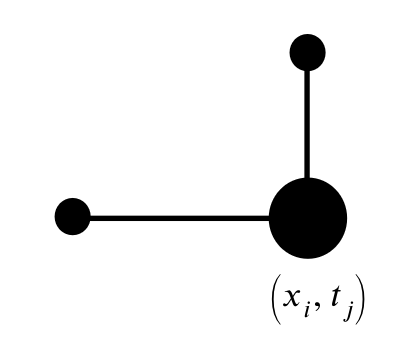
\includegraphics[scale=0.5]{img_1}
    $$
    Используя предложенный шаблон на заданной сетке узлов построим разностную схему в безиндексной форме, заменяя дифференциальные производные разностными аналогами
    \begin{equation}
    	\begin{cases}
    		y_t + ay_{\overline x} = 0,\ (x,t) \in \omega_{h\tau},\\
    		y(x,0) = u_0(x),\ x \in \omega_h.
    	\end{cases}
    \end{equation}
    Разностная схема (2) также может быть записана в индексной форме в виде
    \begin{equation}
    	\begin{dcases}
    		\dfrac{y_k^{j+1} - y_k^j}{\tau} + a \dfrac{y_{k}^j - y_{k-1}^j}{h}=0,\  k=\pm1,\pm 2,\ldots, j = 0,1,2,\ldots,\\
    		y_k^0 = u_0(x),\ k = 0,\pm 1,\ldots.
    	\end{dcases}
    \end{equation}
    Нужно вычислить погрешность аппроксимации разностной схемы. Поскольку мы имеем одно начальное условие, то погрешность аппроксимации всей схемы будет определяться только погрешностью аппроксимации уравнения. Поэтому для любой точки $(x,t) \in \omega_{h\tau}$ погрешность аппроксимации будет равна
    $$\Psi(x,t) = u_t + au_{\overline x} = \dfrac{\d u}{\d t} + \dfrac \tau 2 \dfrac{\d ^2 u}{\d t^2} + O(\tau^2) + a \left(\dfrac{\d u}{\d x} + \dfrac h 2 \dfrac{\d ^2 u}{\d x^2} + O(h^2) \right) = O(h+\tau),$$ то есть данная разностная схема обладает первым порядком аппроксимации по $x$ и первым порядком аппроксимации по $t$.
    \section{Исследование устойчивости разностной схемы спектральным методом}
    Исследование устойчивости по спектральному методу предусматривает подстановку следующего выражения в разностное уравнение
    $$y_k^j = q^j e^{ik\varphi},\ \varphi \in (0, 2\pi).$$
    Итак, подставляя это выражение в разностное уравнение схемы (3), получим
    $$\dfrac{q^{j+1} e^{ik\varphi} - q^j e^{ik\varphi}}{\tau} + a \dfrac{q^j e^{ik\varphi} - q^j e^{i(k-1)\varphi}}{h}=0.$$
    Сокращая общие множители, получим
    $$\dfrac{q - 1}{\tau} + a \dfrac{1 - e^{-i\varphi}}{h} = 0.$$
    Таким образом, можно выразить
    $$q = 1 - \gamma (1 - e^{-i\varphi}),\ \gamma = \dfrac {a\tau}{h}.$$
    Далее по спектральному методу для устойчивости необходимо выполнение условия $|q|^2 \leq 1$. Рассмотрим это условие
    \begin{multline*}
    	|q|^2 = |1 - \gamma(1 - \cos \varphi + i\sin\varphi)|^2 = (1 - \gamma(1-\cos \varphi))^2 + (\gamma \sin\varphi)^2 = \\
    	= 1 - 2\gamma (1-\cos\varphi) + \gamma^2 ( 1-\cos\varphi)^2 + \gamma^2 \sin^2\varphi = 1 -  2\gamma (1-\cos\varphi) + \gamma^2 - 2\gamma^2\cos \varphi + \gamma^2 = \\
    	= 1 - 2\gamma(1-\cos\varphi) + 2 \gamma^2 (1 - \cos\varphi) = 1 + 2\gamma(\gamma - 1)(1-\cos\varphi) \leq 1.
    \end{multline*}
    Отсюда
    $$2\gamma(\gamma - 1)(1-\cos\varphi) \leq 0.$$
    Поскольку $1-\cos\varphi > 0,\ \varphi\in (0,2\pi)$, то получаем систему условий для устойчивости
    \begin{equation}
    	\begin{cases}
    		\gamma \geq 0,\\
    		\gamma \leq 1.
    	\end{cases}
    \end{equation}
    То есть при выполнении условий (4) разностная схема будет устойчива по спектральному методу.\\\\
    Подставляя известное нам значение $a=1$, получим, что
    $$0 \leq \dfrac \tau h \leq 1,$$
    или
    $$0 \leq \tau \leq h.$$
    \section{Исследование устойчивости разностной схемы с помощью принципа максимума}
    Следуя принципу максимума, в качестве точки для исследования устойчивости возьмем точку $(x_i, t_{j+1})$. Таким образом, мы можем переписать аппроксимацию основного уравнения переноса
    $$\dfrac{1}{\tau} y_k^{j+1} = \left(\dfrac{1}{\tau} - \dfrac a h\right)y_k^j + \dfrac a hy_{k-1}^j.$$
    Можем записать коэффициенты, которые требуются для проверки условий устойчивости
    $$A(x) = \dfrac 1 \tau,\ B_1 = \dfrac 1 \tau - \dfrac a h,\ B_2 = \dfrac a h,$$
    $$D(x) = A(x) - (B_1 + B_2) \equiv 0,\ F(x)\equiv 0.$$
    Проверим, выполняются ли соответствующие условия устойчивости:
    $$A(x) = \dfrac 1 \tau > 0, B_1 = \dfrac 1 \tau - \dfrac a h \geq 0,\ B_2 = \dfrac a h > 0,$$
    причем второе условие выполняется, когда из условия $B_1 \geq 0$ следует, что $\dfrac {a\tau } h \leq 1$, или, что то же самое, \begin{equation}
    	\tau \leq \dfrac h a,
    \end{equation}
    называемое условием Куранта.
    \\\\
    Подставляя известное нам значение $a=1$, получим, что
    $$\tau \leq h.$$
    Таким образом, мы можем считать, что условия устойчивости полученные по спектральному методу и по принципу максимума, совпадают.
    \section{Машинная реализация разностной схемы}
    
    

    
    Подключим необходимые библиотеки для работы с векторами и визуализации

    \begin{tcolorbox}[breakable, size=fbox, boxrule=1pt, pad at break*=1mm,colback=cellbackground, colframe=cellborder]
\prompt{In}{incolor}{1}{\boxspacing}
\begin{Verbatim}[commandchars=\\\{\}]
\PY{k+kn}{import} \PY{n+nn}{numpy} \PY{k}{as} \PY{n+nn}{np}
\PY{k+kn}{import} \PY{n+nn}{matplotlib}\PY{n+nn}{.}\PY{n+nn}{pyplot} \PY{k}{as} \PY{n+nn}{plt}
\PY{k+kn}{import} \PY{n+nn}{seaborn} \PY{k}{as} \PY{n+nn}{sns}
\end{Verbatim}
\end{tcolorbox}

    Определим функцию для генерации сеток узлов. Она имеет следующие
параметры:

\begin{itemize}
\item
  left\_border : левая граница сетки;
\item
  right\_border : правая граница сетки;
\item
  num\_x\_points : число разбиений по \(x\);
\item
  upper\_bound : верхняя граница сетки;
\item
  num\_t\_points : число разбиений по \(t\).
\end{itemize}

В результате функция возвращает значения:

\begin{itemize}
\item
  nodes\_x : сетка узлов \(\omega_h\);
\item
  nodes\_t : сетка узлов \(\omega_\tau\);
\item
  h : шаг по \(x\);
\item
  tau : шаг по \(t\).
\end{itemize}

    \begin{tcolorbox}[breakable, size=fbox, boxrule=1pt, pad at break*=1mm,colback=cellbackground, colframe=cellborder]
\prompt{In}{incolor}{2}{\boxspacing}
\begin{Verbatim}[commandchars=\\\{\}]
\PY{k}{def} \PY{n+nf}{generate\PYZus{}grids}\PY{p}{(}\PY{n}{left\PYZus{}border}\PY{p}{,} \PY{n}{right\PYZus{}border}\PY{p}{,} \PY{n}{num\PYZus{}x\PYZus{}points}\PY{p}{,} \PY{n}{upper\PYZus{}bound}\PY{p}{,} \PY{n}{num\PYZus{}t\PYZus{}points}\PY{p}{)}\PY{p}{:}

  \PY{n}{h} \PY{o}{=} \PY{p}{(}\PY{n}{right\PYZus{}border}\PY{o}{\PYZhy{}}\PY{n}{left\PYZus{}border}\PY{p}{)} \PY{o}{/} \PY{n}{num\PYZus{}x\PYZus{}points}
  \PY{n}{nodes\PYZus{}x} \PY{o}{=} \PY{n}{np}\PY{o}{.}\PY{n}{linspace}\PY{p}{(}\PY{n}{left\PYZus{}border}\PY{p}{,} \PY{n}{right\PYZus{}border}\PY{p}{,} \PY{n}{num\PYZus{}x\PYZus{}points}\PY{o}{+}\PY{l+m+mi}{1}\PY{p}{)}

  \PY{n}{tau} \PY{o}{=} \PY{n}{upper\PYZus{}bound} \PY{o}{/} \PY{n}{num\PYZus{}t\PYZus{}points}
  \PY{n}{nodes\PYZus{}t} \PY{o}{=} \PY{n}{np}\PY{o}{.}\PY{n}{linspace}\PY{p}{(}\PY{l+m+mi}{0}\PY{p}{,} \PY{n}{upper\PYZus{}bound}\PY{p}{,} \PY{n}{num\PYZus{}t\PYZus{}points}\PY{o}{+}\PY{l+m+mi}{1}\PY{p}{)}

  \PY{n+nb}{print}\PY{p}{(}\PY{l+s+s1}{\PYZsq{}}\PY{l+s+s1}{h =}\PY{l+s+s1}{\PYZsq{}}\PY{p}{,} \PY{n}{h}\PY{p}{)}
  \PY{n+nb}{print}\PY{p}{(}\PY{l+s+s1}{\PYZsq{}}\PY{l+s+s1}{tau =}\PY{l+s+s1}{\PYZsq{}}\PY{p}{,} \PY{n}{tau}\PY{p}{)}

  \PY{k}{return} \PY{n}{nodes\PYZus{}x}\PY{p}{,} \PY{n}{nodes\PYZus{}t}\PY{p}{,} \PY{n}{h}\PY{p}{,} \PY{n}{tau}
\end{Verbatim}
\end{tcolorbox}

    Определим функцию \[u(x,t) = u_0(x-at),\] соответствующую точному
решению поставленной задачи Коши. Зададим \(a=1\) и \(u_0(x) = x^2\).

    \begin{tcolorbox}[breakable, size=fbox, boxrule=1pt, pad at break*=1mm,colback=cellbackground, colframe=cellborder]
\prompt{In}{incolor}{3}{\boxspacing}
\begin{Verbatim}[commandchars=\\\{\}]
\PY{k}{def} \PY{n+nf}{u}\PY{p}{(}\PY{n}{x}\PY{p}{,} \PY{n}{t}\PY{p}{,} \PY{n}{a}\PY{p}{,} \PY{n}{u\PYZus{}0}\PY{p}{)}\PY{p}{:}
    \PY{k}{return} \PY{n}{u\PYZus{}0}\PY{p}{(}\PY{n}{x}\PY{o}{\PYZhy{}}\PY{n}{a}\PY{o}{*}\PY{n}{t}\PY{p}{)}

\PY{n}{a} \PY{o}{=} \PY{l+m+mi}{1}
\PY{k}{def} \PY{n+nf}{u\PYZus{}0}\PY{p}{(}\PY{n}{x}\PY{p}{)}\PY{p}{:}
    \PY{k}{return} \PY{n}{x}\PY{o}{*}\PY{o}{*}\PY{l+m+mi}{2}
\end{Verbatim}
\end{tcolorbox}

    Определим функцию, реализующую вычисление по разностной схеме в
соответствии с рекуррентной формулой \[\begin{cases}
            y_k^{j+1} = (1-\gamma)y_k^j + \gamma y_{k+1}^j,\ k = 0\pm1,\pm2\ldots,\ j = 0,1,\ldots,\\
            y_k^0 = u_0(x_k),\ k = 0,\pm 1,\ldots.
        \end{cases}\quad \gamma = \dfrac {a\tau}{h}.
\] В результате функция возвращает матрицу \(y\), где каждая строка это
приближенное решение в каждой точке \(x\) в момент времени \(t\), а
столбцы -- это моменты \(t\).

    \begin{tcolorbox}[breakable, size=fbox, boxrule=1pt, pad at break*=1mm,colback=cellbackground, colframe=cellborder]
\prompt{In}{incolor}{4}{\boxspacing}
\begin{Verbatim}[commandchars=\\\{\}]
\PY{k}{def} \PY{n+nf}{diff\PYZus{}scheme\PYZus{}solve}\PY{p}{(}\PY{n}{nodes\PYZus{}x}\PY{p}{,} \PY{n}{nodes\PYZus{}t}\PY{p}{,} \PY{n}{h}\PY{p}{,} \PY{n}{tau}\PY{p}{,} \PY{n}{u\PYZus{}0}\PY{p}{,} \PY{n}{a}\PY{p}{)}\PY{p}{:}
    \PY{n}{gamma} \PY{o}{=} \PY{n}{a} \PY{o}{*} \PY{n}{tau} \PY{o}{/} \PY{n}{h}

    \PY{n}{y} \PY{o}{=} \PY{n}{np}\PY{o}{.}\PY{n}{zeros}\PY{p}{(}\PY{p}{(}\PY{n+nb}{len}\PY{p}{(}\PY{n}{nodes\PYZus{}x}\PY{p}{)}\PY{p}{,} \PY{n+nb}{len}\PY{p}{(}\PY{n}{nodes\PYZus{}t}\PY{p}{)}\PY{p}{)}\PY{p}{)}

    \PY{k}{for} \PY{n}{k} \PY{o+ow}{in} \PY{n+nb}{range}\PY{p}{(}\PY{n+nb}{len}\PY{p}{(}\PY{n}{nodes\PYZus{}x}\PY{p}{)}\PY{p}{)}\PY{p}{:}
        \PY{n}{y}\PY{p}{[}\PY{n}{k}\PY{p}{,} \PY{l+m+mi}{0}\PY{p}{]} \PY{o}{=} \PY{n}{u\PYZus{}0}\PY{p}{(}\PY{n}{nodes\PYZus{}x}\PY{p}{[}\PY{n}{k}\PY{p}{]}\PY{p}{)}

    \PY{k}{for} \PY{n}{k} \PY{o+ow}{in} \PY{n+nb}{range}\PY{p}{(}\PY{n+nb}{len}\PY{p}{(}\PY{n}{nodes\PYZus{}x}\PY{p}{)}\PY{o}{\PYZhy{}}\PY{l+m+mi}{1}\PY{p}{)}\PY{p}{:}
      \PY{k}{for} \PY{n}{j} \PY{o+ow}{in} \PY{n+nb}{range}\PY{p}{(}\PY{n+nb}{len}\PY{p}{(}\PY{n}{nodes\PYZus{}t}\PY{p}{)}\PY{o}{\PYZhy{}}\PY{l+m+mi}{1}\PY{p}{)}\PY{p}{:}
            \PY{n}{y}\PY{p}{[}\PY{n}{k}\PY{p}{,} \PY{n}{j}\PY{o}{+}\PY{l+m+mi}{1}\PY{p}{]} \PY{o}{=} \PY{p}{(}\PY{l+m+mi}{1}\PY{o}{\PYZhy{}}\PY{n}{gamma}\PY{p}{)} \PY{o}{*} \PY{n}{y}\PY{p}{[}\PY{n}{k}\PY{p}{,} \PY{n}{j}\PY{p}{]} \PY{o}{+} \PY{n}{gamma} \PY{o}{*} \PY{n}{y}\PY{p}{[}\PY{n}{k}\PY{o}{+}\PY{l+m+mi}{1}\PY{p}{,} \PY{n}{j}\PY{p}{]}

    \PY{k}{return} \PY{n}{y}
\end{Verbatim}
\end{tcolorbox}

    Определим следующие сетки узлов. Пусть \(x \in [0,1]\), а отрезок
\([0,1]\) разобъем на 5 частей. Пусть \(t \in [0, 0.25]\), а отрезок
\([0, 0.25]\) разобъем на 5 частей. Таким образом, получим следующие
шаги \(h\) и \(\tau\).

    \begin{tcolorbox}[breakable, size=fbox, boxrule=1pt, pad at break*=1mm,colback=cellbackground, colframe=cellborder]
\prompt{In}{incolor}{5}{\boxspacing}
\begin{Verbatim}[commandchars=\\\{\}]
\PY{n}{nodes\PYZus{}x}\PY{p}{,} \PY{n}{nodes\PYZus{}t}\PY{p}{,} \PY{n}{h}\PY{p}{,} \PY{n}{tau} \PY{o}{=} \PY{n}{generate\PYZus{}grids}\PY{p}{(}\PY{l+m+mi}{0}\PY{p}{,} \PY{l+m+mi}{1}\PY{p}{,} \PY{l+m+mi}{5}\PY{p}{,} \PY{l+m+mf}{0.25}\PY{p}{,} \PY{l+m+mi}{5}\PY{p}{)}
\end{Verbatim}
\end{tcolorbox}

    \begin{Verbatim}[commandchars=\\\{\}]
h = 0.2
tau = 0.05
    \end{Verbatim}

    По нашим математическим обоснованиям данная разностная схема должна быть
устойчива.

Вычислим значения приближенного решения \(y\) по разностной схеме.

    \begin{tcolorbox}[breakable, size=fbox, boxrule=1pt, pad at break*=1mm,colback=cellbackground, colframe=cellborder]
\prompt{In}{incolor}{6}{\boxspacing}
\begin{Verbatim}[commandchars=\\\{\}]
\PY{n}{y} \PY{o}{=} \PY{n}{diff\PYZus{}scheme\PYZus{}solve}\PY{p}{(}\PY{n}{nodes\PYZus{}x}\PY{p}{,} \PY{n}{nodes\PYZus{}t}\PY{p}{,} \PY{n}{h}\PY{p}{,} \PY{n}{tau}\PY{p}{,} \PY{n}{u\PYZus{}0}\PY{p}{,} \PY{n}{a}\PY{p}{)}
\end{Verbatim}
\end{tcolorbox}

    Построим визуализацию полученных результатов. На графике представлены
точное и приближенное решение.

    \begin{tcolorbox}[breakable, size=fbox, boxrule=1pt, pad at break*=1mm,colback=cellbackground, colframe=cellborder]
\prompt{In}{incolor}{7}{\boxspacing}
\begin{Verbatim}[commandchars=\\\{\}]
\PY{k}{for} \PY{n}{j}\PY{p}{,} \PY{n}{t} \PY{o+ow}{in} \PY{n+nb}{enumerate}\PY{p}{(}\PY{n}{nodes\PYZus{}t}\PY{p}{)}\PY{p}{:}
  \PY{n}{plt}\PY{o}{.}\PY{n}{figure}\PY{p}{(}\PY{n}{figsize}\PY{o}{=}\PY{p}{(}\PY{l+m+mi}{16}\PY{p}{,} \PY{l+m+mi}{8}\PY{p}{)}\PY{p}{)}
  \PY{n}{plt}\PY{o}{.}\PY{n}{plot}\PY{p}{(}\PY{n}{nodes\PYZus{}x}\PY{p}{[}\PY{p}{:}\PY{o}{\PYZhy{}}\PY{l+m+mi}{1}\PY{p}{]}\PY{p}{,} \PY{n}{y}\PY{p}{[}\PY{p}{:}\PY{o}{\PYZhy{}}\PY{l+m+mi}{1}\PY{p}{,} \PY{n}{j}\PY{p}{]}\PY{p}{,} \PY{n}{label}\PY{o}{=}\PY{l+s+s1}{\PYZsq{}}\PY{l+s+s1}{numerical solution}\PY{l+s+s1}{\PYZsq{}}\PY{p}{)}
  \PY{n}{plt}\PY{o}{.}\PY{n}{plot}\PY{p}{(}\PY{n}{nodes\PYZus{}x}\PY{p}{,} \PY{n}{u}\PY{p}{(}\PY{n}{nodes\PYZus{}x}\PY{p}{,} \PY{n}{t}\PY{p}{,} \PY{n}{a}\PY{p}{,} \PY{n}{u\PYZus{}0}\PY{p}{)}\PY{p}{,} \PY{n}{label}\PY{o}{=}\PY{l+s+s1}{\PYZsq{}}\PY{l+s+s1}{exact solution}\PY{l+s+s1}{\PYZsq{}}\PY{p}{)}
  \PY{n}{plt}\PY{o}{.}\PY{n}{grid}\PY{p}{(}\PY{k+kc}{True}\PY{p}{)}
  \PY{n}{plt}\PY{o}{.}\PY{n}{xlabel}\PY{p}{(}\PY{l+s+s1}{\PYZsq{}}\PY{l+s+s1}{x}\PY{l+s+s1}{\PYZsq{}}\PY{p}{)}
  \PY{n}{plt}\PY{o}{.}\PY{n}{ylabel}\PY{p}{(}\PY{l+s+s1}{\PYZsq{}}\PY{l+s+s1}{u(x,t)}\PY{l+s+s1}{\PYZsq{}}\PY{p}{)}
  \PY{n}{plt}\PY{o}{.}\PY{n}{title}\PY{p}{(}\PY{l+s+s1}{\PYZsq{}}\PY{l+s+s1}{Approximation in t\PYZus{}}\PY{l+s+s1}{\PYZsq{}} \PY{o}{+} \PY{n+nb}{str}\PY{p}{(}\PY{n}{j}\PY{p}{)} \PY{o}{+} \PY{l+s+s1}{\PYZsq{}}\PY{l+s+s1}{=}\PY{l+s+s1}{\PYZsq{}} \PY{o}{+} \PY{n+nb}{str}\PY{p}{(}\PY{n+nb}{round}\PY{p}{(}\PY{n}{t}\PY{p}{,} \PY{l+m+mi}{2}\PY{p}{)}\PY{p}{)}\PY{p}{)}
  \PY{n}{plt}\PY{o}{.}\PY{n}{legend}\PY{p}{(}\PY{p}{)}
  \PY{n}{plt}\PY{o}{.}\PY{n}{show}\PY{p}{(}\PY{p}{)}
\end{Verbatim}
\end{tcolorbox}

    \begin{center}
    \adjustimage{max size={0.9\linewidth}{0.9\paperheight}}{output_13_0.png}
    \end{center}
    { \hspace*{\fill} \\}
    
    \begin{center}
    \adjustimage{max size={0.9\linewidth}{0.9\paperheight}}{output_13_1.png}
    \end{center}
    { \hspace*{\fill} \\}
    
    \begin{center}
    \adjustimage{max size={0.9\linewidth}{0.9\paperheight}}{output_13_2.png}
    \end{center}
    { \hspace*{\fill} \\}
    
    \begin{center}
    \adjustimage{max size={0.9\linewidth}{0.9\paperheight}}{output_13_3.png}
    \end{center}
    { \hspace*{\fill} \\}
    
    \begin{center}
    \adjustimage{max size={0.9\linewidth}{0.9\paperheight}}{output_13_4.png}
    \end{center}
    { \hspace*{\fill} \\}
    
    \begin{center}
    \adjustimage{max size={0.9\linewidth}{0.9\paperheight}}{output_13_5.png}
    \end{center}
    { \hspace*{\fill} \\}
    
    Действительно, построенное по разностной решение приближенно описывает
точное решение поставленной дифференциальной задачи. То есть схема
действительно оказалась устойчивой.

    Определим следующие сетки узлов. Пусть \(x \in [0,1]\), а отрезок
\([0,1]\) разобъем на 5 частей. Пусть \(t \in [0, 2]\), а отрезок
\([0, 2]\) разобъем на 5 частей. Таким образом, получим следующие шаги
\(h\) и \(\tau\).

    \begin{tcolorbox}[breakable, size=fbox, boxrule=1pt, pad at break*=1mm,colback=cellbackground, colframe=cellborder]
\prompt{In}{incolor}{9}{\boxspacing}
\begin{Verbatim}[commandchars=\\\{\}]
\PY{n}{nodes\PYZus{}x}\PY{p}{,} \PY{n}{nodes\PYZus{}t}\PY{p}{,} \PY{n}{h}\PY{p}{,} \PY{n}{tau} \PY{o}{=} \PY{n}{generate\PYZus{}grids}\PY{p}{(}\PY{l+m+mi}{0}\PY{p}{,} \PY{l+m+mi}{1}\PY{p}{,} \PY{l+m+mi}{5}\PY{p}{,} \PY{l+m+mi}{2}\PY{p}{,} \PY{l+m+mi}{5}\PY{p}{)}
\PY{n}{y} \PY{o}{=} \PY{n}{diff\PYZus{}scheme\PYZus{}solve}\PY{p}{(}\PY{n}{nodes\PYZus{}x}\PY{p}{,} \PY{n}{nodes\PYZus{}t}\PY{p}{,} \PY{n}{h}\PY{p}{,} \PY{n}{tau}\PY{p}{,} \PY{n}{u\PYZus{}0}\PY{p}{,} \PY{n}{a}\PY{p}{)}
\end{Verbatim}
\end{tcolorbox}

    \begin{Verbatim}[commandchars=\\\{\}]
h = 0.2
tau = 0.4
    \end{Verbatim}

    Такая разностная схема должна быть неустойчивой. Рассмотрим графики
решений

    \begin{tcolorbox}[breakable, size=fbox, boxrule=1pt, pad at break*=1mm,colback=cellbackground, colframe=cellborder]
\prompt{In}{incolor}{10}{\boxspacing}
\begin{Verbatim}[commandchars=\\\{\}]
\PY{k}{for} \PY{n}{j}\PY{p}{,} \PY{n}{t} \PY{o+ow}{in} \PY{n+nb}{enumerate}\PY{p}{(}\PY{n}{nodes\PYZus{}t}\PY{p}{)}\PY{p}{:}
  \PY{n}{plt}\PY{o}{.}\PY{n}{figure}\PY{p}{(}\PY{n}{figsize}\PY{o}{=}\PY{p}{(}\PY{l+m+mi}{16}\PY{p}{,} \PY{l+m+mi}{8}\PY{p}{)}\PY{p}{)}
  \PY{n}{plt}\PY{o}{.}\PY{n}{plot}\PY{p}{(}\PY{n}{nodes\PYZus{}x}\PY{p}{[}\PY{p}{:}\PY{o}{\PYZhy{}}\PY{l+m+mi}{1}\PY{p}{]}\PY{p}{,} \PY{n}{y}\PY{p}{[}\PY{p}{:}\PY{o}{\PYZhy{}}\PY{l+m+mi}{1}\PY{p}{,} \PY{n}{j}\PY{p}{]}\PY{p}{,} \PY{n}{label}\PY{o}{=}\PY{l+s+s1}{\PYZsq{}}\PY{l+s+s1}{numerical solution}\PY{l+s+s1}{\PYZsq{}}\PY{p}{)}
  \PY{n}{plt}\PY{o}{.}\PY{n}{plot}\PY{p}{(}\PY{n}{nodes\PYZus{}x}\PY{p}{,} \PY{n}{u}\PY{p}{(}\PY{n}{nodes\PYZus{}x}\PY{p}{,} \PY{n}{t}\PY{p}{,} \PY{n}{a}\PY{p}{,} \PY{n}{u\PYZus{}0}\PY{p}{)}\PY{p}{,} \PY{n}{label}\PY{o}{=}\PY{l+s+s1}{\PYZsq{}}\PY{l+s+s1}{exact solution}\PY{l+s+s1}{\PYZsq{}}\PY{p}{)}
  \PY{n}{plt}\PY{o}{.}\PY{n}{grid}\PY{p}{(}\PY{k+kc}{True}\PY{p}{)}
  \PY{n}{plt}\PY{o}{.}\PY{n}{xlabel}\PY{p}{(}\PY{l+s+s1}{\PYZsq{}}\PY{l+s+s1}{x}\PY{l+s+s1}{\PYZsq{}}\PY{p}{)}
  \PY{n}{plt}\PY{o}{.}\PY{n}{ylabel}\PY{p}{(}\PY{l+s+s1}{\PYZsq{}}\PY{l+s+s1}{u(x,t)}\PY{l+s+s1}{\PYZsq{}}\PY{p}{)}
  \PY{n}{plt}\PY{o}{.}\PY{n}{title}\PY{p}{(}\PY{l+s+s1}{\PYZsq{}}\PY{l+s+s1}{Approximation in t\PYZus{}}\PY{l+s+s1}{\PYZsq{}} \PY{o}{+} \PY{n+nb}{str}\PY{p}{(}\PY{n}{j}\PY{p}{)} \PY{o}{+} \PY{l+s+s1}{\PYZsq{}}\PY{l+s+s1}{=}\PY{l+s+s1}{\PYZsq{}} \PY{o}{+} \PY{n+nb}{str}\PY{p}{(}\PY{n+nb}{round}\PY{p}{(}\PY{n}{t}\PY{p}{,} \PY{l+m+mi}{2}\PY{p}{)}\PY{p}{)}\PY{p}{)}
  \PY{n}{plt}\PY{o}{.}\PY{n}{legend}\PY{p}{(}\PY{p}{)}
  \PY{n}{plt}\PY{o}{.}\PY{n}{show}\PY{p}{(}\PY{p}{)}
\end{Verbatim}
\end{tcolorbox}

    \begin{center}
    \adjustimage{max size={0.9\linewidth}{0.9\paperheight}}{output_20_0.png}
    \end{center}
    { \hspace*{\fill} \\}
    
    \begin{center}
    \adjustimage{max size={0.9\linewidth}{0.9\paperheight}}{output_20_1.png}
    \end{center}
    { \hspace*{\fill} \\}
    
    \begin{center}
    \adjustimage{max size={0.9\linewidth}{0.9\paperheight}}{output_20_2.png}
    \end{center}
    { \hspace*{\fill} \\}
    
    \begin{center}
    \adjustimage{max size={0.9\linewidth}{0.9\paperheight}}{output_20_3.png}
    \end{center}
    { \hspace*{\fill} \\}
    
    \begin{center}
    \adjustimage{max size={0.9\linewidth}{0.9\paperheight}}{output_20_4.png}
    \end{center}
    { \hspace*{\fill} \\}
    
    \begin{center}
    \adjustimage{max size={0.9\linewidth}{0.9\paperheight}}{output_20_5.png}
    \end{center}
    { \hspace*{\fill} \\}
    
    Как можно видеть из построенного графика, полученное приближенное
решение сильно отклоняется от точного решения, а также на каждом
временном слое меняет знак. Из этого мы можем заключить, что разностная
схема действительно является неустойчивой.    
    
\end{document}
